		
	
	Dans la figure ci-dessous, on a tracé $C_f$ la courbe représentative d'une fonction $f$ définie et dérivable sur $\mathbb{R}$ ainsi que les tangentes à $C_f$ aux points d'abscisses respectives $-2$, $-1$ et 0.
	
\subsection*{1. Compléter le tableau de valeurs ci-dessous. }
	
	\[
	\begin{array}{|c|c|c|c|}
		\hline	x & -2 & -1 & 0 \\
		\hline
		f(x) & 1 & 1 & 1 \\
		\hline
		f'(x) & 2 & -1 & 2 \\
			\hline
	\end{array}
	\]
	

	\subsection*{2. a. Calculer $f'(x)$, pour tout réel $x$.}
	
	On a sur $\mathbb{R}$, $f'(x) = 3x^2 + 6x + 2$.
	
	\subsubsection*{b. Résoudre dans $\mathbb{R}$ l'équation : $f'(x) = 0$.}
	
	$f'(x) = 0 \iff 3x^2 + 6x + 2 = 0$, \\
	on a $\Delta = 36 - 24 = 12 = (2\sqrt{3})^2 > 0$.
	
	L'équation a donc deux solutions :
	\[
	x_1 = \dfrac{-6 + 2\sqrt{3}}{6} = \dfrac{-3 + \sqrt{3}}{3} \quad \text{et} \quad x_2 = \dfrac{-6 - 2\sqrt{3}}{6} = \dfrac{-3 - \sqrt{3}}{3}
	\]
	
	\subsection*{3. Dresser le tableau de variations de la fonction $f$.}
	
	On sait que $f'(x) > 0$, sauf sur l'intervalle $\left] \dfrac{-3 - \sqrt{3}}{3} ; \dfrac{-3 + \sqrt{3}}{3} \right[$ où $f'(x) < 0$.
	
	Donc $f$ est croissante sauf sur l'intervalle $\left] \dfrac{-3 + \sqrt{3}}{3} ; \dfrac{-3 + \sqrt{3}}{3} \right[$ où elle est décroissante.
	
	\begin{center}
	\begin{tikzpicture}[double distance=2pt]
		\tkzTabInit{$x$/1,$f'(x)$/1,$f(x)$/3}{$-\infty$,$\dfrac{-3 - \sqrt{3}}{3}$,$\dfrac{-3 + \sqrt{3}}{3}$, $+\infty$}
		\tkzTabLine{,+,z,-,z, +}
		\tkzTabVar{-/,+/$1+\dfrac{2\sqrt3}{9}$,-/$1-\dfrac{2\sqrt3}{9}$,+/}
	\end{tikzpicture}
\end{center} 


	
	\subsection*{4. Le point $S(-4 ; -3)$ appartient-il à la tangente à la courbe représentative de $f$ au point d'abscisse $x = -2$ ?}
	
	Équation de la tangente au point $(-2 ; f(-2))$.
	
	On a $f(-2) = (-2)^3 + 3 \times (-2)^2 + 2 \times (-2) + 1 = -8 + 12 - 4 + 1 = 1$.
	
	$f'(-2) = 3 \times (-2)^2 + 6 \times (-2) + 2 = 2$.
	
	La tangente $(T)$ en $S$ a pour équation :
	\begin{align*}
&	M(x ; y) \in (T)\\
	 \iff& y - f(-2) = f'(-2)(x - (-2))\\
	 \iff& y - 1 = 2(x + 2)\\
	 \iff& y = 2x + 4 + 1 \\
	\iff &y = 2x + 5
	\end{align*}
	
	Donc $S(-4 ; -3) \in (T) \iff -3 = 2 \times (-4) + 5 \iff -3 = -8 + 5$ qui est vraie.
	
